% !TeX spellcheck = en_GB
\def\ChapterTitle{Assessment of TMF Performance in Marine Environments}

\ifx\ifthesis\undefined
\documentclass[a4paper, 11pt]{article}

% % Special Includes stolen from Thesis.cls
\usepackage{booktabs}
\usepackage{hyperref}
\usepackage{graphicx}
\usepackage{epstopdf}
\usepackage{subcaption}
\usepackage{rotating}
\usepackage{listings}
\usepackage{lstpatch}
\renewcommand{\arraystretch}{1.3}

% % % % % % % % % % % % % % % %

% PACKAGES
\usepackage[square, numbers, comma, sort&compress]{natbib}  % Use the "Natbib" style for the references in the Bibliography
\usepackage{verbatim,listings}  % Needed for the "comment" environment to make LaTeX comments
\usepackage{array}  % Needed for the "comment" environment to make LaTeX comments
\usepackage{vector}  % Allows "\bvec{}" and "\buvec{}" for "blackboard" style bold vectors in maths
\usepackage{amsmath,amsfonts,amsthm,color,psfrag,epsf, tabularx, multirow, longtable}
\usepackage{snapshot, todonotes}
% \usepackage{pstricks}
\usepackage{enumerate}
%\usepackage[lined,algonl,boxed]{algorithm2e}
\usepackage[ruled,linesnumbered,vlined]{algorithm2e}
\usepackage{float}
\usepackage{epigraph} % epigraph
\usepackage{tikz}
\usetikzlibrary{shapes.geometric, arrows}

\usepackage{setspace}
\doublespacing
% or:
%\onehalfspacing

% SETUP
\hypersetup{urlcolor=blue, colorlinks=false}  % Colours hyperlinks in blue, but this can be distracting if there are many links. 
\DeclareGraphicsExtensions{.pdf,.jpeg,.png}
\graphicspath{{../Figures/}{../../../Dropbox/Thesis_Figures/}}  % Location of the graphics files (set up for graphics to be in PDF format)

% NOTE THERES A FUCKUP IN TEX4HT http://tug.org/pipermail/tex4ht/2014q2/000944.html
% NEED TO MANUALLY CHANGE \def\pgfsys@svg@newline{{?nl}}
\ifdefined\HCode
\usepackage[compatibility=false]{caption}
\def\pgfsysdriver{pgfsys-tex4ht.def}
\else
\usepackage[]{caption}
\fi

% \SpecialCoor
\def\subsum{\mathit{\Sigma}}

%opening
\title{\ChapterTitle}
\author{Andrew Bolster}

\begin{document}

\maketitle

\else
\chapter{\ChapterTitle}
\label{Chapter\thechapter}
\lhead{Chapter \thechapter. \emph{\nameref{Chapter\thechapter}}} % Write in your own chapter title to set the page header
\fi



\section{Comparison of Terrestrial and Marine Communication Trust Assessments}

In this chapter, we demonstrate the need for multi-metric trust assessment in Underwater Autonomous Networks (UAN).
Many UANs use MANET architectures, however the marine environment presents new challenges for trust management frameworks that have been developed for use in conventional (i.e. Terrestrial RF) MANETs.
We investigate the operation of a selection of traditional MANET TMFs in this environment.
We characterise these challenges and present results that demonstrate a multi-metric approach to Trust greatly enhances the effectiveness of TMFs in these environments.

\subsection{Trust in Marine Networks}\label{sec:trust_in_marine}

With demand for smaller, more decentralised marine survey and monitoring systems, and a drive towards lower per-unit cost, TMFs are going to be increasingly applied to the marine space, as the benefits they present are significant.
Beyond the constraints of the communications environment, knock on pressures are applying in battery capacity, on-board processing, and locomotion.
These pressures simultaneously present opportunities and incentives for malicious or selfish actors to appear to cooperate while not reciprocating, in order to conserve power for instance.
These multiple aspects of potential incentives, trust, and fairness do not directly fall under the scope of single metric trusts discussed above, and this context indicates that a multi-metric approach may be more appropriate.

As mobile ad-hoc networks (MANETs) grow beyond the terrestrial arena, their operation and the protocols designed around them must be reviewed to assess their suitability to different communications environments to ensure their continued security, reliability, and performance.

One area of application is the underwater marine environment, where extreme challenges to communications present themselves (propagation delays, frequency dependent attenuation, fast and slow fading, refractive multi-path distortion, etc.).
In addition to the communications challenges, other considerations such as command and control isolation, as well as power and locomotive limitations, drive towards the use of teams of smaller and cheaper autonomous underwater vehicles (AUVs). 
These increasingly decentralised applications present unique threats against trust management \cite{Caiti2011}.
In underwater environments, communications is both sparse and noisy.
Therefore the observations about the communications processes that are used to generate the trust metrics, occur much less frequently, with much greater error (noise) and delay than is experienced in terrestrial RF MANETS.
As such, the use of trust methods developed in the terrestrial MANET space must be re-appraised for application within the underwater context \cite{Pavan2015}.

Trust Management Frameworks (TMFs) provide information to assist the estimation of future states and actions of nodes within networks.
This information is used to optimize the performance of a network against malicious, selfish, or defective misbehaviour by one or more nodes.
Previous research has established the advantages of implementing TMFs in 802.11 based MANETs, particularly in terms of preventing selfish operation in collaborative systems \cite{Li2007}, and maintaining throughput in the presence of malicious actors \cite{Buchegger2002}

Most current TMFs use a single type of observed action to derive trust values, typically successfully delivered or forwarded packets. 
These observations then inform future decisions of individual nodes, for example, route selection \cite{Li2008}.

Recent work has demonstrated the use of a number of metrics to form a ``vector'' of trust.
The Multi-parameter Trust Framework for MANETs (MTFM) \cite{Guo11}, uses a range of communications metrics beyond packet delivery/loss rate (PLR) to assess trust.
This vectorized trust also allows a system to detect and identify the tactics being used to undermine or subvert trust.
To date this work has been limited to terrestrial, RF based networks. 

\subsection{Establishing Scale Factors in Communications Rate}

In this section we characterise the simulated communications environment, establishing an optimal packet emission rate for comparison against \cite{Guo11}.

In order to establish the point at which the network becomes saturated due, a range of packet emission rates were explored between 0.01 packets per second (pps), equivalent to 96 bps, up to 0.07 pps (672 bps)

From Figs.~\ref{fig:throughput_performance_static} and ~\ref{fig:prod_breakdown_static}, it is clear that the threshold curve, expressed as the \emph{Successfully Received Packets} line, exhibits a saturation point between 0.025 and 0.03 pps.
Particularly in Fig.~\ref{fig:prod_breakdown_static}, the precipitous drop in packet delivery probability beyond 0.025 pps, indicating that this is a strong candidate value for an upper-limit to the safe operating zone in terms of packet emission in the small static case.

\begin{figure}[H]
	\centering
	%\missingfigure{throughput_performance_static}
	\caption{Varying packet emission rate demonstrates maximal throughput at 0.025 packets per second, equivalent to $\approx$240 bps}
	\label{fig:3d}
\end{figure}


\begin{figure}[H]
	\centering
	%\missingfigure{prod_breakdown_static}
	\caption{Varying packet emission rate demonstrates a saturation point at 0.025 packets per second}
	\label{fig:prod_breakdown_static}
\end{figure}



\subsection{Establishing Scale Factors in Physical Distribution}

In this section we characterise the effect of node-separation scaling on communications operation for comparison against \cite{Guo11}. This is particularly important considering the significant scale factor differences between not only the speed of propagation in the medium, but simply the range of operation. 
From Table \ref{tab:sysconstraints}, the operating transmission range of acoustic is $\approx 6$ times further than 802.11, indicating that a suitable operating environment will have an area $\approx \sqrt{6}$ times the area of the 802.11 case. Therefore, a reasonable experimental range would have an upper bound of performance around this scaling factor, where nodes are approximately 400$m$ apart. 

A reasonable range around this is to scale from 100$m$ apart on average to 800$m$.

Varying average node separation shows that while direct throughput isn't significantly affected until, collision rates are Fig.~\ref{fig:throughput_performance_range}.
This collision rate is well within the tolerances of the MAC layer, as shown in Fig.~\ref{fig:prod_breakdown_range}, where even with a rising collision rate, packets are being reliably received.

\begin{figure}[H]
	\centering
	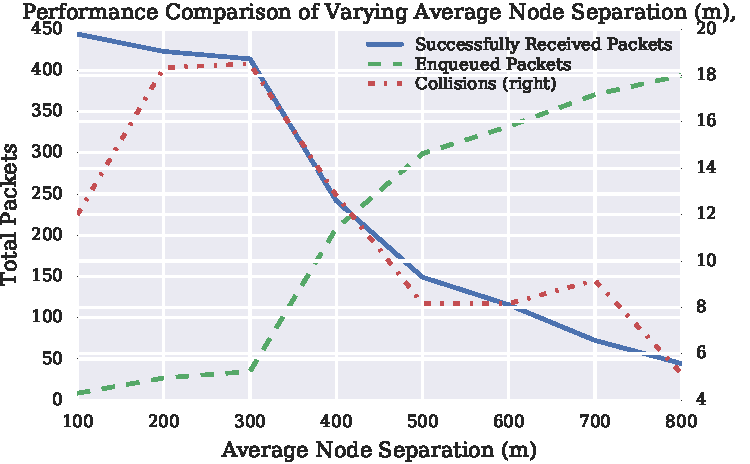
\includegraphics[width=0.6\textwidth]{throughput_performance_range}
	\caption{Comparison of Medium Acquisition Collisions, Throughput, and Enqueued packets against varying application packet emission rates.}
	\label{fig:throughput_performance_range}
\end{figure}

\begin{figure}[H]
	\centering
	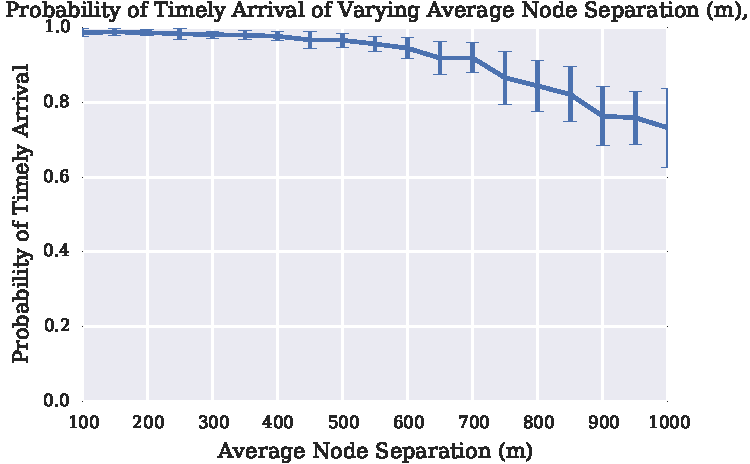
\includegraphics[width=0.6\textwidth]{prod_breakdown_range.pdf}
	\caption{Probability of Timely Reception across a range of node scaling.}
	\label{fig:prod_breakdown_range}
\end{figure}

However, when end-to-end delay is investigated, it's clear from Fig.~\ref{fig:delay_range} that the network is becoming severely impaired approaching the 600$m$ mark, with delays rising to more than 25 minutes above 700$m$.
This is also demonstrated by the increasing RTS/Data ratio shown in Fig.~\ref{fig:rts_range}.

According to Xu \cite{Xu2002}, the RTS/CTS handshake cannot function well as interference protection at node separations beyond 0.56 times the transmission range. 
This is also demonstrated in  Fig.~\ref{fig:rts_range}, where above $1500m \times 0.56 = 840m$, 
This is due to reduced channel availability due to collisions, which are then due to a much longer potential contention period between nodes. 

\begin{figure}[H]
	\centering
	\missingfigure{delay range}
	%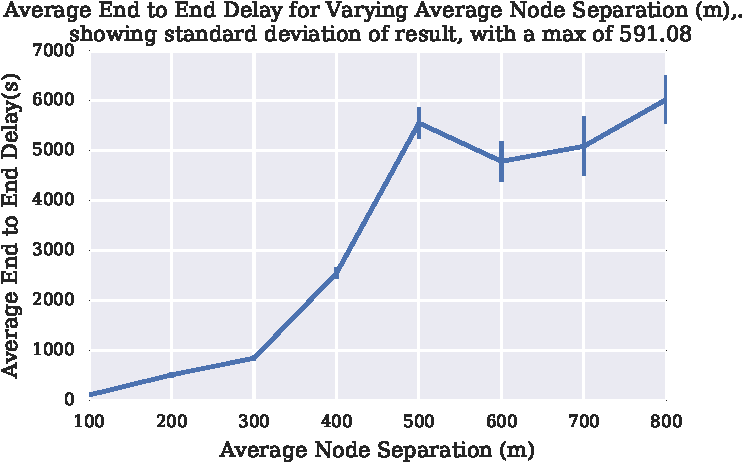
\includegraphics[width=0.6\textwidth]{delay_range}
	\caption{End to End Delay under varying node-separations}
	\label{fig:delay_range}
\end{figure}

\begin{figure}[H]
	\centering
	\missingfigure{rts range}
	%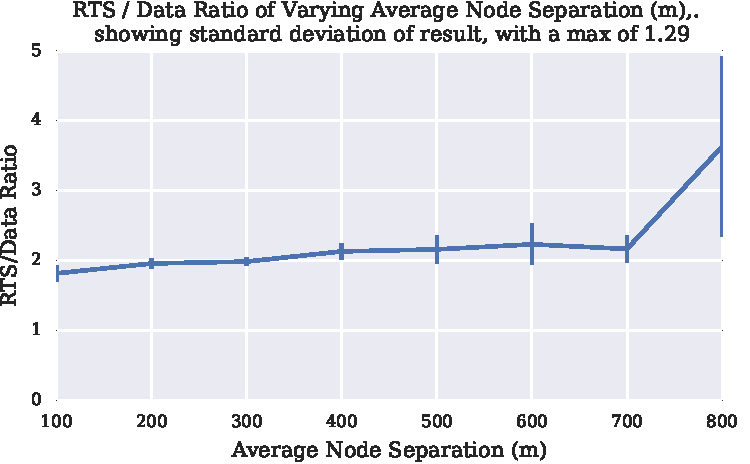
\includegraphics[width=0.6\textwidth]{rts_range}
	\caption{RTS/Data ratio for varying node-separations}
	\label{fig:rts_range}
\end{figure}


\begin{table}[H]
	\caption{Tabular view of data from Figs~\ref{fig:prod_breakdown_range}, \ref{fig:delay_range}, and \ref{fig:rts_range}} \label{tab:rangedelay}
	\begin{center}
		\hyphenpenalty 100000
		\begin{tabular}{
				*{2}{@{\hspace{1em}}r@{\hspace{1em}}}
				*{3}{@{\hspace{1em}}p{0.1\textwidth} @{\hspace{1em}}}  }
			\toprule
			Separation(m) &  Delay(s) &  Probability of Arrival &  RTS/Data Ratio &  Ideal Delivery Time(s) \\
			\midrule
			100 &     60.32 &                    0.99 &            1.80 &                    1.03 \\
			200 &    419.95 &                    0.97 &            2.02 &                    1.10 \\
			300 &   1205.66 &                    0.89 &            2.41 &                    1.17 \\
			400 &   1288.20 &                    0.91 &            2.26 &                    1.25 \\
			500 &   1868.20 &                    0.87 &            2.41 &                    1.32 \\
			600 &   2191.07 &                    0.85 &            2.42 &                    1.39 \\
			\bottomrule
		\end{tabular}
	\end{center}
\end{table}
